\documentclass{article}
\usepackage{lipsum}
\usepackage[utf8]{inputenc}
\usepackage{amsmath, amssymb, graphicx}
\usepackage{tikz}
\usepackage{multicol}
\usepackage[hidelinks]{hyperref}
\usepackage{cite}
\usepackage{caption}
\usepackage{multirow}
\usepackage{adjustbox}

%%%%%%%%%%%%%%%% Lengths %%%%%%%%%%%%%%%%
\setlength{\textwidth}{16.5cm}
\setlength{\evensidemargin}{-0.5cm}
\setlength{\oddsidemargin}{-0.5cm}
\setlength{\topmargin}{-1.5cm}
\setlength{\textheight}{23cm}

%%%%%%%%%%%%%%%% Variables %%%%%%%%%%%%%%%%
\def\projet{1}
\def\titre{Limites de la représentation des nombres flottants}
\def\groupe{4}
\def\equipe{3}
\def\responsible{Mélissa Colin}
\def\secretary{Mohamed Aziz Migaou}
\def\others{Younes Bamouss, Anna Gouedard}
\graphicspath{{img/}}
\begin{document}

%%%%%%%%%%%%%%%% Header %%%%%%%%%%%%%%%%
\noindent\begin{minipage}{0.98\textwidth}
  \vskip 0mm
  \noindent
  { \begin{tabular}{p{7cm}}
      {\bfseries \sffamily
        Projet \projet} \\ 
      {\itshape \titre}
    \end{tabular}}
  \hfill 
  \fbox{\begin{tabular}{l}
      {~\hfill \bfseries \sffamily Groupe \groupe\ - Equipe \equipe
        \hfill~} \\[2mm] 
      Responsable : \responsible \\
      Secrétaire : \secretary \\
      Codeurs : \others
    \end{tabular}}
  \vskip 4mm ~

  ~~~\parbox{0.95\textwidth}{\small \textit{Résumé~:} \sffamily Ce travail étudie les limites de la représentation des nombres flottants en machine, en mettant en évidence les erreurs d'arrondi et les imprécisions associées. Nous analysons les erreurs relatives dans les opérations arithmétiques fondamentales et implémentons des algorithmes numériques pour le calcul du logarithme népérien et des fonctions trigonométriques en utilisant la méthode CORDIC. Les résultats montrent l'importance de comprendre ces erreurs pour garantir la fiabilité des calculs en informatique.
    }
  \vskip 1mm ~
\end{minipage}

%%%%%%%%%%%%%%%% Main part %%%%%%%%%%%%%%%%
\section{Introduction}
% Les ordinateurs manipulent les nombres sous forme binaire en mémoire, mais nous étudions ici une approche où ils sont représentés en base 10 avec une précision définie. Nous allons implémenter des fonctions en Python pour simuler ces représentations et étudier les erreurs associées aux opérations.

\subsection{Contexte}
Dans les ordinateurs, les nombres réels ne peuvent pas être représentés avec une précision infinie. Ils sont stockés sous forme de nombres \textit{flottants}, ce qui peut entraîner des erreurs d’arrondi et des imprécisions. La norme IEEE 754 définit les formats et méthodes pour l'arithmétique des nombres à virgule flottante en environnement de programmation informatique \cite{ieee754-2019}. La Figure \ref{fig:ieee754} illustre la représentation des nombres flottants selon cette norme.

\begin{figure}[h]
\centering
\begin{tikzpicture}
  % Sign bit
  \draw[fill=red!20] (1,0) rectangle (2.5,1);
  \node at (1.75,0.5) {Signe};
  \node at (1.75,-0.3) {1 bit};

  % Exponent bits
  \draw[fill=blue!20] (2.5,0) rectangle (5,1);
  \node at (3.75,0.5) {Exposant};
  \node at (3.75,-0.3) {8 bits};

  % Mantissa bits
  \draw[fill=green!20] (5,0) rectangle (12,1);
  \node at (8.5,0.5) {Mantisse};
  \node at (8.5,-0.3) {23 bits};
\end{tikzpicture}
\caption{Schéma de la représentation des nombres flottants (32 bits) selon la norme IEEE 754.}
\label{fig:ieee754}
\end{figure}

\subsection{Motivation}
L’étude de la représentation des nombres et des erreurs qu'elle engendre est essentielle pour garantir la fiabilité des calculs en informatique. Dans de nombreux domaines comme la simulation numérique, le calcul haute performances ou encore l’intelligence artificielle, il est crucial de comprendre comment les erreurs de représentation peuvent affecter les résultats.\\
Ce projet vise donc à anticiper les limites des nombres flottants et à fournir des outils pour analyser ces erreurs.


\section{Méthodologie}
Nous étudions dans un premier temps la représentation décimale réduite des nombres ainsi que l'impact de ses arrondis sur les opérations arithmétiques élémentaires. Puis afin de mieux comprendre les erreurs d'arrondi et de précision, nous avons implémenté des algorithmes numériques pour le calcul du logarithme népérien et des fonctions trigonométriques.


\subsection{Représentation décimale réduite}
Afin d'étudier cette représentation, nous avons réalisé une fonction $rp(x, p)$ en python qui prend un nombre réel $x$ et le représente avec $p$ chiffres significatifs.\\
Pour ce faire, nous avons choisi d'utiliser le module \textit{decimal} en définissant la précision avec \texttt{getcontext().prec = p}.\\ \\
Nous avons en suite simulée l’addition et la multiplication avec ses représentations réduites en calculant l'erreur relative pour chaque opération avec les formules (\ref{eq:relative_error_sum}) et (\ref{eq:relative_error_product}).\\
\vspace{-0.8cm}
\begin{multicols}{2}
\vspace{-0.5cm}
\begin{equation}
\delta_s(x,y) = \frac{|(x + y) - (x_{m} +_{m} y_{m})|}{|x + y|}
\label{eq:relative_error_sum}
\end{equation}
\vspace{0.5cm}
\begin{equation}
\delta_p(x,y) = \frac{|(x \times y) - (x_{m} \times_{m} y_{m})|}{|x \times y|}
\label{eq:relative_error_product}
\end{equation}
\end{multicols}
\textit{\noindent Si on note respectivement  $x$ et $y$ les nombres réels et $x_m$ et $y_m$ leurs représentations machine ainsi que $+_{m}$ et $\times_{m}$ les opératio
ns machine.}\\ \\
Pour visualiser l'impact de la précision sur les opérations arithmétiques, nous avons représenté les erreurs relatives des opérations d'addition et de multiplication en fixant $x =1$ et en faisant varier $y$ en puissance de 10 négatives. L'objectif étant de faire croître la différence d'échelle entre $x$ et $y$.

\subsection{Algorithmes Numériques}
Pour éprouver ses représentations, nous proposons deux algorithmes pour le calcul : l'un utilisant la série entière pour calculer log(2), et l'autre utilisant l'algorithme CORDIC sur quatre fonctions ln, exp, tan et arctan.
\subsubsection{Série entière}
Nous tentons de calculer une valeur approchée de \( \log(2) \) en utilisant une série alternée définie par l'équation \ref{eq:log2_series}.
\begin{equation}
S_n = \sum_{k=1}^{n} \frac{(-1)^{k+1}}{k}
\label{eq:log2_series}
\end{equation}
Cette série est connue pour converger vers \( \log(2) \) lorsque \( n \to \infty \)~\cite{friedli_analyse1}.\\
% Elle constitue une approximation efficace de \( \log(2) \) comme le montre la figure \ref{fig:diffirence absolue}

% \begin{figure}[!ht]
%     \centering
%     \includegraphics[width=\textwidth, height=6cm, keepaspectratio]{img/diff_abs.png}
%     \caption{Différence absolue entre la somme partielle et log(2)}
%     \label{fig:diffirence absolue}
% \end{figure}
\noindent On utilise donc cette approche pour calculer \(\log(2)\) à \(p\) décimales: nous calculons la somme partielle \( S_n \) de la série jusqu'à ce que le terme suivant \( T_{n+1}=\frac{(-1)^{n+2}}{n+1} \) soit inférieur à la précision souhaitée. C'est à dire tant que \( |T_n| = \frac{1}{n} > \epsilon, \quad \text{où} \quad \epsilon = 10^{-p-2} \).

\subsubsection{Algorithme CORDIC}
L'algorithme CORDIC est une méthode de calcul utilisée principalement dans les calculatrices~\cite{volder1959cordic}. Celui-ci utilise pour un nombre flottant 8 octets de mémoire en utilisant une mantisse codée sur 4 chiffres binaires, un exposant signé ou non sous forme d'une puissance de 10 et du signe du nombre.~\cite{usenetMathsFAQ}. Cette méthode permet d'effectuer efficacement diverses opérations mathématiques telles que les fonctions trigonométriques, logarithmiques, et exponentielles, en utilisant uniquement des opérations arithmétiques de base qui réduisent progressivement la valeur de x à une valeur très faible tout en élaborant le résultat, ce qui la rend particulièrement adaptée aux systèmes à ressources limitées. Chacune de ces transformations nécessite une valeur précalculée de la fonction f (ou de son inverse). Cet algorithme possède comme variant la valeur x, un réel qu'on souhaiterait calculer avec une précision d'environ 12 décimales. Dans ce travail, on l'évalue par les fonctions ln, tan et leur bijection réciproque. \\ \\
% On dispose de deux tableaux des valeurs préliminaires de arctan et ln.\ref{tab:tableaux}.

% \noindent
% \begin{center}
% \begin{tabular}{cccc}
% \hline
% $x = 1+10^{-k}$ & $\ln(x)$ & $x = 10^{-k}$ & $\arctan(x)$ \\
% \hline
% 2 & 0,693147180560 & 1 & 0.7853981 \\
% 1,1 & 0,095310179804 & 0,1 & 0.0996687 \\
% 1,01 & 0,009950330853 & 0,01 & 0.00999967 \\
% 1,001 & 0,000999500333 & 0,001 & 0.001 \\
% 1,0001 & 0,000099995000 & 0,0001 & 0,0001 \\
% 1,00001 & 0,000009999950 & -- & -- \\
% 1,000001 & 0,000000999999 & -- & -- \\
% \hline
% \end{tabular}
% \captionof{table}{Les deux tableaux L et A initialisés pour l'algorithme CORDIC}
% \label{tab:tableaux}
% \end{center}

\noindent \textbf{Logarithme népérien et exponentielle}\\
Pour calculer la valeur des fonctions exponentielle et logarithme naturel, nous avons écrit $x$ sous les deux formes suivantes \ref{eq:ln_product} et \ref{eq:exp_sum} pour les fonctions ln et exp respectivement.\\
\begin{equation}
x = \prod_{k=0}^6 \left(1+\frac{1}{10^k}\right)^{n_k} \cdot (1+\varepsilon)
\label{eq:ln_product}
\end{equation}
\begin{equation}
x = \sum_{k=0}^6 n_k \ln\left(1+\frac{1}{10^k}\right) + \varepsilon
\label{eq:exp_sum}
\end{equation}
Avec $n_0, n_1, \ldots, n_6$ des coefficients maximaux et $\varepsilon \leq 10^{-7}$ (Cela est dû aux coefficients maximaux).\\ \\
Le logarithme vérifie la propriété suivante $\forall x,y \in \mathbf{R}^{+*} \ln(xy)=\ln(x)+\ln(y)$. On a donc :
\begin{equation}
\ln(x) = \ln\left(\prod_{k=0}^6 \left(1+\frac{1}{10^k}\right)^{n_k}\right) + \ln(1+\varepsilon) = \sum_{k=0}^6 n_k \ln\left(1+\frac{1}{10^k}\right) + \ln(1+\varepsilon) = \sum_{k=0}^6 n_k L[k] + \ln(1+\varepsilon)
\label{eq:ln_final}
\end{equation}

Or $\varepsilon \leq 10^{-7}$, et $\ln(1+x) \sim x$ et $e^x \sim x+1$  quand $x \to 0$. donc :
\begin{equation}
\boxed{\ln(x)=\sum_{k=0}^6 n_k L[k] + \varepsilon}
\quad
\boxed{e^x = (1+\varepsilon) \prod_{k=0}^6 \left(1+\frac{1}{10^k}\right)^{n_k}}
\label{eq:exp_final}
\end{equation}
\\
\textbf{Tangente et Arctangente}\\
Pour calculer les valeurs des fonctions trigonométriques \( \tan \) et \( \arctan \), nous utilisons les relations suivantes. La relation pour \( \arctan \) est donnée par l'équation \ref{eq:arctan_relation} et pour \( \tan \) par l'équation \ref{eq:tan_relation}.
\begin{equation}
\arctan\left(\frac{x}{y}\right)=\arctan\left(\frac{x-y\cdot10^{-k}}{y+x\cdot10^{-k}}\right)+\arctan(10^{-k})
\label{eq:arctan_relation}
\end{equation}
\textit{Avec initialement \( x = x \), \( y = 1 \), et \( k \leq 4 \). En appliquant la relation d'équivalence \( \arctan(x) \sim x \) lorsque \( x \to 0 \), on obtient l'équation \ref{eq:arctan}.}
\begin{equation}
\arctan(x) = \sum_{k=0}^4 n_k \cdot A[k] + \varepsilon
\label{eq:arctan}
\end{equation}
\textit{où \( 0 \leq \varepsilon \leq 10^{-4} \).}

\begin{equation}
\tan\left(s - \arctan(10^{-k})\right) = \frac{n}{d} \quad \Rightarrow \quad \tan(s) = \frac{n + d \cdot 10^{-k}}{d - n \cdot 10^{-k}}
\label{eq:tan_relation}
\end{equation}
\textit{car  $\tan(a-b) = \frac{\tan a - \tan b}{1 + \tan a \tan b}$. En utilisant le fait que $\tan$ est impaire et $\tan(x) \sim x$ lorsque $x \sim 0$, on considère "$0 \leq s$" est un invariant de l'algorithme donc s est diminue (terminaison) dans:}
\begin{equation}
\tan(s)=\frac{n+d\cdot10^{-k}}{d-n\cdot10^{-k}}
\label{eq:tan}
\end{equation}

\section{Résultats et discussions}
Dans cette section, nous présentons et analysons les résultats obtenus à partir des différentes méthodes et algorithmes implémentés. \\
Nous commencerons par discuter des résultats relatifs à la représentation décimale réduite, en mettant en évidence les erreurs relatives observées lors des opérations d'addition et de multiplication. Ensuite, nous analyserons les performances des algorithmes numériques, en évaluant leur précision et leur efficacité pour les calculs de fonctions mathématiques spécifiques.
\subsection{Représentation décimale réduite}
\noindent En traçant le graphique, visible en figure~\ref{fig:relative_error}, on observe d'importantes différences entre l'addition et la multiplication.
\begin{figure}[h]
  \centering
  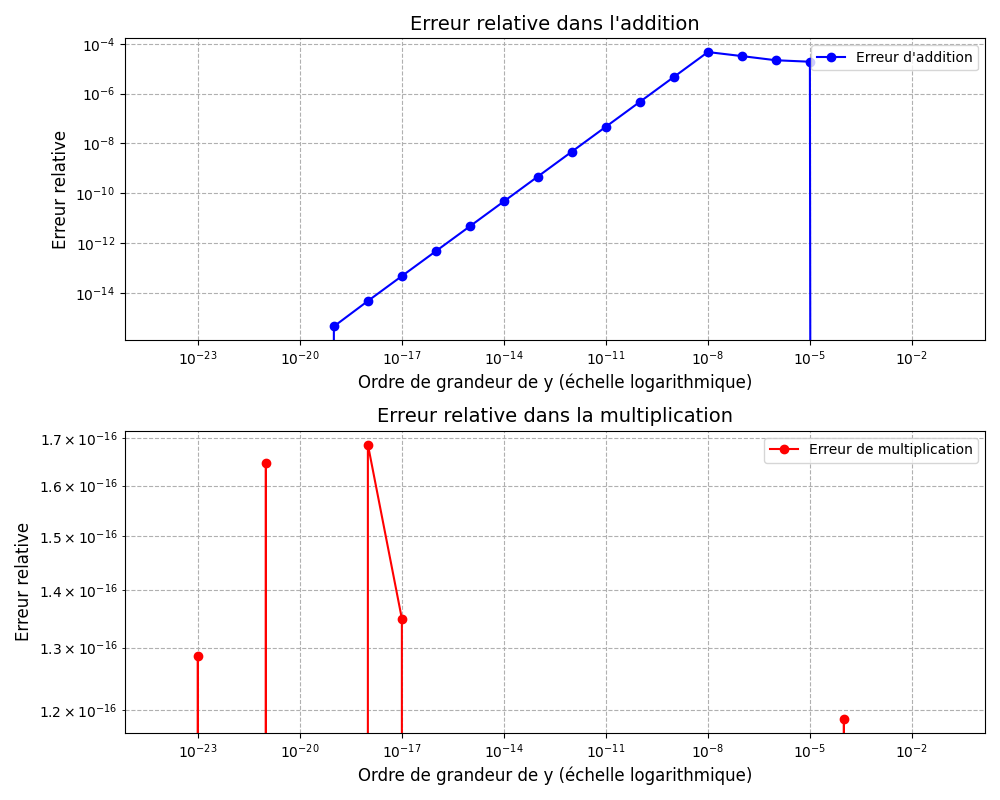
\includegraphics[width=0.9\textwidth]{img/relativ_error.png}
\caption{Erreurs relatives sur l'addition (en bleu) et la multiplication (en rouge) avec une précision $p = 5$ pour $x = 1$ et $y$ décroissant en puissances de 10 sur une échelle logarithmique.}
  \label{fig:relative_error}
\end{figure}
\begin{itemize}
    \item L'erreur relative dans l'addition augmente progressivement avec $y$. Pour des valeurs très petites de $y$ (ex. $y < 10^{-20}$), l'erreur est négligeable car $y$ est trop petit pour influencer la somme. Cependant, à partir de $y \approx 10^{-17}$, elle croît de manière quasi linéaire en échelle logarithmique jusqu’à un maximum, ce qui correspond à un phénomène de perte de précision dû à l’arrondi numérique. Ce phénomène est particulièrement visible lorsque deux nombres de grandeurs très différentes sont additionnés. À partir de $y \approx 10^{-5}$, l'erreur atteint un plateau proche de $10^{-4}$, montrant que la précision est limitée par la représentation décimale réduite.
    
    \item L'erreur relative dans la multiplication reste globalement stable autour de $1.6 \times 10^{-16}$, ce qui correspond aux limites de précision imposées par la norme IEEE 754 pour les nombres flottants en double précision. Contrairement à l'addition, la multiplication est moins affectée par la différence d’ordre de grandeur entre $x$ et $y$, expliquant cette stabilité. On observe toutefois de légères fluctuations, qui sont dues aux effets de l’arrondi numérique.

\end{itemize}
L'analyse des erreurs relatives montre que l'addition est plus sujette à des pertes de précision que la multiplication, en particulier lorsque les nombres manipulés diffèrent fortement en ordre de grandeur.
\subsection{Algorithmes Numériques}
Ces résultats montrent l'importance de comprendre les erreurs d'arrondi et de précision dans les calculs numériques. Pour approfondir cette analyse, nous avons mis en œuvre des algorithmes spécifiques afin d'évaluer leur impact sur des fonctions mathématiques couramment utilisées. Les sections suivantes présentent les détails des résultats obtenus pour chaque algorithme.

\subsubsection{Série entière}
Lors des tests de l'algorithme de la série entière pour le calcul de \( \log(2) \), nous avons remarqué que plus la valeur de \( p \) augmente, plus l'algorithme met de temps à s'exécuter en raison de la convergence particulièrement lente de la série harmonique alternée. Par exemple, pour \( p = 6 \), la somme doit inclure jusqu’au terme \( n = 100000001 \), ce qui entraîne un temps d’attente considérable. 

\subsubsection{Algorithme CORDIC}
En testant les quatre fonctions sur les entiers de 1 à 300, on observe que les fonctions \( \ln \) et \( \arctan \) offrent une bonne précision pour les valeurs comprises entre 1 et 300 comme présenté dans le tableau~\ref{tab:precision_results}). Alors que \( \exp \) et \( \tan \) peuvent atteindre jusqu'à 9 chiffres significatifs. 
\begin{table}[h!]
\centering
\begin{tabular}{|c|c|c|c|}
\hline
\textbf{Fonction} & \textbf{Précision} & \textbf{Nombre de valeurs} & \textbf{Pourcentage de valeurs} \\
\hline
\multirow{2}{*}{$\ln$} 
& 11 décimales & 2 & 0,67\% \\
& $\geq$12 décimales & 298 & 99,33\% \\
\hline
\multirow{2}{*}{$\exp$} 
& 9 décimales & 2 & 0,67\% \\
& 10 décimales & 4 & 1,33\% \\
& 11 décimales & 59 & 19,67\% \\
& $\geq$12 décimales & 235 & 78,33\% \\
\hline
\multirow{3}{*}{$\tan$} 
& 10 décimales & 10 & 3,33\% \\
& 11 décimales & 41 & 13,67\% \\
& $\geq$12 décimales & 249 & 83,00\% \\
\hline
\multirow{2}{*}{$\arctan$} 
& 11 décimales & 1 & 0,33\% \\
& $\geq$12 décimales & 299 & 99,67\% \\
\hline
\end{tabular}
\caption{Pourcentage de valeurs ayant une certaine précision pour $\ln$, $\exp$, $\tan$ et $\arctan$ entre 1 et 300}
\label{tab:precision_results}
\end{table}
\\\\ Pour \( \exp \), avec une précision d'ordre \( 6 \) (\( \ln(1 + 10^{-6}) = 0.00000099 \)) et la relation d'équivalence, la précision est d'environ 12 chiffres après la virgule \(\frac{\exp(10^{-6})}{10^{-6} + 1} = 1.0000000000004999\) , tandis que pour \( \tan \), avec une précision d'ordre \( 4 \) (\( \arctan(10^{-4}) = 0.0001 \)), la relation d'équivalence donne une précision d'environ 9 chiffres après la virgule \(\frac{\tan(10^{-4})}{10^{-4}} = 1.0000000033333334\).
\section{Conclusion et perspectives}
Ce travail a permis de mettre en évidence les limites de la représentation des nombres flottants en machine. Les erreurs d’arrondi deviennent problématiques lorsque les nombres manipulés ont des ordres de grandeur très différents. D'autre part, elles sont plus marquées dans l'addition que dans la multiplication, ce qui met en évidence la sensibilité accrue de cette opération aux effets de la précision flottante. Les résultats sont cohérents avec la mise en évidence des limites de la précision flottante IEEE 754 étudiée en classe.\\
En mettant en œuvre des algorithmes numériques, nous avons pu calculer des valeurs approchées de fonctions mathématiques en utilisant des méthodes de calcul alternatives. Les résultats obtenus montrent que ces algorithmes peuvent être efficaces pour obtenir des approximations précises de fonctions mathématiques. Cependant, des séries à convergence plus rapide pourraient être utilisées pour surmonter ce problème et réduire significativement le temps d'exécution.

%%%%%%%%%%%%%%%% Bibliography %%%%%%%%%%%%%%%%
\bibliographystyle{plain}
\bibliography{references}
\end{document}